\begin{mdframed}[style=warning]
	\begin{ejercicio}
		\textbf{Conceptos.}
		\begin{enumerate}
			\item Sus manos están húmedas y el dispensador de toallas del baño está vacío. ¿Qué hace para quitar las gotas de agua de sus manos? ¿Cómo su acción ejemplifica una de las leyes de Newton? ¿Cuál de ellas?
			\item ¿Un objeto puede ejercer una fuerza sobre sí mismo? Argumente.
			\item Una cubeta de agua se puede girar en una trayectoria vertical tal que no se derrame agua. ¿Por qué el agua permanece en la cubeta, aun cuando la cubeta esté sobre su cabeza?
			\item ¿Por qué un piloto tiende a desmayarse cuando sale de una pronunciada caída en picada?
		\end{enumerate}
	\end{ejercicio}
\end{mdframed}





\begin{mdframed}[style=warning]
	\begin{ejercicio}
		El bloque $A$, de peso $3w$, se desliza con rapidez constante, bajando por un plano $S$ inclinado $36.9^o$, mientras la tabla $B$, de peso $w$, descansa sobre $A$, estando sujeta con una cuerda a la pared. Si el coeficiente de fricción es igual entre $A$ y $B$ y entre $S$ y $A$, determine su valor.
		\begin{figure}[H]
			\centering
			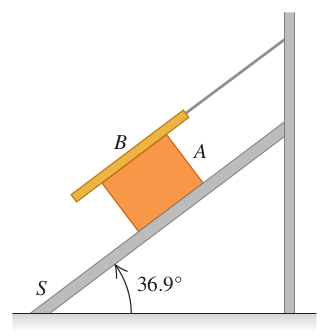
\includegraphics[scale=0.35]{./img/599.png}
			\caption{Ejercicio 2}
			\label{599}
		\end{figure}
	\end{ejercicio}
\end{mdframed}







\begin{mdframed}[style=warning]
	\begin{ejercicio}
		Una cuenta pequeña puede desliarse sin fricción por un aro circular de $0.1m$ de radio, que está e un plano vertical. El aro gira con velocidad constante de $4rev/s$ en torno a un diametro vertical. \textit{(a)} Calcule el ángulo $\beta$ en el que la cuenta está en equilibrio vertical. \textit{(b)} ¿La cuenta podría permanecer a la misma altura que el centro del aro?
		\begin{figure}[H]
			\centering
			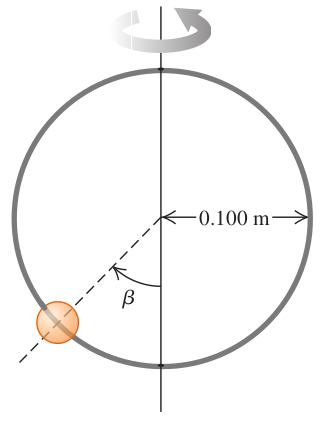
\includegraphics[scale=0.35]{./img/5119.png}
			\caption{Ejercicio 3}
			\label{5119}
		\end{figure}
	\end{ejercicio}
\end{mdframed}

















\begin{mdframed}[style=warning]
	\begin{ejercicio}
		Si un bloque cuadrado se desliza por una cuña con ángulo recto inclinada un ángulo $\theta$. El coeficiente de fricción cinético entre la cuña y el bloque es $\mu _k$. ¿Cuál es la aceleración del bloque en términos de las variables conocidas?
		\begin{figure}[H]
			\centering
			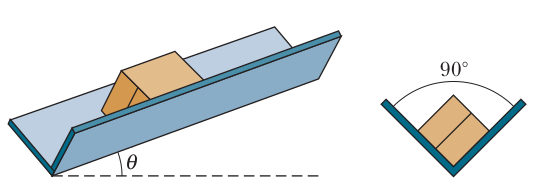
\includegraphics[scale=0.3]{./img/cuna.png}
			\caption{Ejercicio 4}
		\end{figure}
	\end{ejercicio}
\end{mdframed}








\begin{mdframed}[style=warning]
	\begin{ejercicio}
		Un bloque pequeño de masa $m$ se coloca dentro de un cono invertido que gira sobre un eje vertical, de modo que la duración de una revolución del cono es $T$. La pared del cono forma un ángulo $\beta$ con la horizontal. El coeficiente de fricción estática entre el bloque y el cono es $\mu _s$. Si el bloque debe mantenerse a una altura constante $h$ sobre el vértice del cono. ¿Cuáles son el valor máximo y mínimo de $T$?
	\end{ejercicio}
\end{mdframed}









\begin{mdframed}[style=warning]
	\begin{ejercicio}
		En la figura se muestra un sistema mecánico que consiste en tres carritos, $A$, $B$ y $C$ de masas $m_1$, $m_2$ y $m_3$ respectivamente. Los carros $A$ y $B$ estan conectados por una cuerda ligera e inelástica que pasa por una polea ideal fijada en $C$. Para este problema se ignora la fuerza de fricción.
	\begin{enumerate}
		\item Una fuerza horizontal $\vec{F}$ es aplicada al carro $C$. El tamaño de $\vec{F}$ es tal qeu los carritos $A$ y $B$ se mantienen en reposo respecto al carro $C$.
		\begin{enumerate}[a)]
			\item Encuentre la tensión de la cuerda que conecta los carritos $A$ y $B$.
			\item Determine la magnitud de $\vec{F}$.
		\end{enumerate}
		\item Luego, el carro $C$ se detiene. Mientras que los carritos $A$ y $B$ se sueltan desde el reposo.
		\begin{enumerate}[a)]
			\item Determine las aceleraciones de los carritos $A$ y $B$.
			\item Calcule la tensión de la cuerda.
		\end{enumerate}
	\end{enumerate}
		\begin{figure}[H]
			\centering
			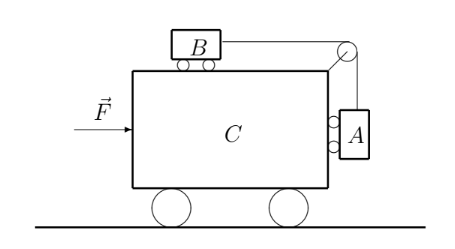
\includegraphics[scale=0.4]{./img/carrito.png}
			\caption{Ejercicio 6}
		\end{figure}
	\end{ejercicio}
\end{mdframed}





\begin{mdframed}[style=warning]
	\begin{reto}
		Un prisma triangular de masa $M$ se encuentra en un plano horizontal sin fricción. Los otros dos lados del prisma están inclinados respecto al plano unos ángulos $\alpha _1$ y $\alpha _2$ respectivamente. Dos bloques de masa $m_1$ y $m_2$, conectados por unna cuerda inelástica que pasa por una polea ideal.
	\begin{itemize}
		\item Exprese la aceleración $a$ de los bloques relativas al prisma en términos de la aceleración $a_o$ del prisma.
		\item Encuentre la aceleración $a_o$ del prisma en términos de las cantidades conocidas.
		\item ¿A qué razón $m_1 /m_2$ el prisma estará en equilibrio?
	\end{itemize}
		\begin{figure}[H]
			\centering
			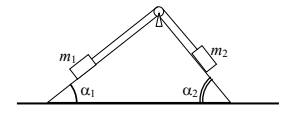
\includegraphics[scale=0.7]{./img/cunamovil.png}
			\caption{Reto.}
		\end{figure}
	\end{reto}
\end{mdframed}


















%%%